
% Packages

\documentclass[conference]{IEEEtran}
\IEEEoverridecommandlockouts
\usepackage{epsfig}

\usepackage{graphicx}   % A package for graphics use (see figures)

\usepackage{cite}

\usepackage{booktabs}

\usepackage{balance}  % for  \balance command ON LAST PAGE  (only there!)
\usepackage{amsmath}
\usepackage{xspace}
\usepackage{subfigure}
%\usepackage{bibspacing}
\usepackage{url}
\usepackage{float}
%\usepackage{pslatex}

\usepackage[algoruled,vlined,linesnumbered,commentsnumbered]{algorithm2e}


\usepackage{comment}

\newcommand{\inlineitem}[1]{\vspace{1ex}\noindent{\bf {#1}}}
\newcommand{\closeinlineitem}{\vspace{1ex}}
\newcommand{\specialcell}[2][l]{ \begin{tabular}[#1]{@{}l@{}}#2\end{tabular}}

\newif\ifremark
\long\def\remark#1{
\ifremark%
	\begingroup%
	\dimen0=\columnwidth
	\advance\dimen0 by -0.25in%
	\setbox0=\hbox{\parbox[b]{\dimen0}{\protect\em #1}}
	\dimen1=\ht0\advance\dimen1 by 2pt%
	\dimen2=\dp0\advance\dimen2 by 2pt%
	\vskip 0.25pt%
	\hbox to \columnwidth{%
		\vrule height\dimen1 width 3pt depth\dimen2%
		\hss\copy0\hss%
		\vrule height\dimen1 width 3pt depth\dimen2%
	}%
	\endgroup%
\fi}

\remarktrue

\newcommand{\eg}{{\em e.g.}, }
\newcommand{\ie}{{\em i.e.}, }
\newcommand{\etal}{{\em et al.\ }}

\pagestyle{empty}


\begin{document}
\IEEEoverridecommandlockouts
\IEEEpubid{\makebox[\columnwidth]{978-1-5090-3216-7/16/\$31.00~\copyright{}2016 IEEE \hfill}\hspace{\columnsep}\makebox[\columnwidth]{ }}

%\title{Reducing communication cost of similarity based encrypted data search with compressed bloom filters}
\title{Reducing Communication Cost of Encrypted Data Search with Compressed Bloom Filters}

\author{

\IEEEauthorblockN{
	Muhammad Umer\IEEEauthorrefmark{1},
	Tahir Azim\IEEEauthorrefmark{1}\IEEEauthorrefmark{2} and 
	Zeeshan Pervez\IEEEauthorrefmark{3}
}
\IEEEauthorblockA{\IEEEauthorrefmark{1} National University of Sciences and Technology (NUST), Islamabad, Pakistan}
\IEEEauthorblockA{\IEEEauthorrefmark{2} \'{E}cole Polytechnique F\'{e}d\'{e}rale de Lausanne, Switzerland}
\IEEEauthorblockA{\IEEEauthorrefmark{3} University of the West of Scotland, Paisley, Scotland PA1 2BE} 
Email: 13msitmumer@seecs.edu.pk, tahir.azim@epfl.ch, zeeshan.pervez@uws.ac.uk
}

\maketitle

\begin{abstract}

Consumer data, such as documents, photos and videos, are increasingly being
stored in the cloud. To ensure confidentiality of the data, it is oustourced after encryption. However, this makes it difficult to search the encrypted data 
directly. Recent approaches to enable searching of this encrypted data
have relied on trapdoors, locally stored indexes, and homomorphic encryption.
However, data communication cost for these techniques are very high and they limit search capabilities either to a small set of 
pre-defined trapdoors or only allow exact keyword matching.

This paper addresses the problem of high communication cost, similarity-based search over
outsourced encrypted data while ensuring end-to-end privacy. We have proposed a novel compression algorithm by 
avoiding the need to send back the entire encrypted bloom filter index to the 
client. This reduces the cost of communicating results to the client by over 95\%. Our scheme enables users to search using keywords that only partially match the originally stored words.
We implement partial matching using sliding window bloom filters and secure
search over arbitrary keywords using homomorphic encryption.

To demonstrate viability of our scheme we implement it on a real cloud, Google ecosystem, and our results show the reduction in communication cost over 95\% and search queries with 2 to 10 keywords only cost \$0.000002 to \$0.00002 per 1000 similar requests.

\end{abstract}





%% \terms
%% Algorithms, Design, Experimentation, Performance

%% \keywords
%% Virtual worlds, Discovery, Spatial
%\keywordlist

\section{Introduction}

Cloud computing enables its subcscribers to use computing services over the 
Internet and provides tailored computing resources on-demand. 
Subscribers of cloud storage can outsource their data on public cloud servers
without worrying about the availability and
reliability of the data. It is then the cloud service provider's (CSP) 
responsibility to coordinate data backup, synchronization and sharing
with relevant stakeholders. 

As the amount of data stored on the cloud increases dramatically, the security 
of this data has become an important concern. Recent cases have included users'
photos and videos getting stolen from compromised cloud servers resulting in
severe breaches of privacy. Credit card numbers, dates of birth and medical
records are other examples of user data whose privacy needs to be ensured.

The straightforward way to achieve data protection, confidentiality and privacy is to place data on the cloud after encrypting it using public key encryption. 
This solves the confidentiality and privacy problem
but encryption hides data information and searching becomes impossible. The user has to download all
the data from cloud storage and search it after decrypting it locally. This is
obviously an extremely expensive proposition. Therefore we need a mechanism 
which can enable a user to search over the encrypted data without revealing 
private information and without downloading excessive data over the network.

Existing approaches for searching over encrypted data often rely on so-called
"trapdoors". Trapdoors enable a user to search the encrypted data for a small 
set of pre-defined keywords. These approaches restrict the searching
capability of a user to a limited number of trapdoors defined during data 
encryption. More recent work has focused on homomorphic encryption~\cite{craig} as a solution
to this problem. However, to ensure privacy from CSP, all the evaluated results are returned from cloud server without any compression casuing high data communication cost and naively allows searching for exact keyword matches over the encrypted data. 

In this paper, we present a novel system for performing searches on encrypted 
data in the cloud. we proposed a novel compression technique which allows us to avoid sending back the
entire encrypted index back to the client. This reduces the cost of
communicating search results back to the client by over 95\% resulting in 
faster response times and less budeging cost ($) to the owner. In addition to exact keyword matching, our system also
supports similarity-based searching: finding documents with partially matching 
keywords rather than only those with exact keywords. Privacy and search 
capabilities are enabled using homomorphic encryption, while sliding window 
bloom filters allow us to search for partially matching keywords. 

The next section overviews related work in more detail.  Section
\ref{sec:system} presents a detailed description of our system and the 
algorithms it uses.
Section \ref{sec:eval} demonstrates the benefits of using our approaches
on a dataset of encrypted textual data. 
Section \ref{sec:conclusion} then concludes with a treatment of
some implications and trade-offs of using our system.

\section{Related Work}
\label{sec:related}

Traditionally, confidential information is protected using access control
mechanisms. This mechanism only works if confidential information is present on
a fully secure, trusted server. But this assumption fails when confidential 
information is outsourced to remote servers in the cloud.

Although cloud service providers (CSP) allow data to be encrypted in order to 
secure it, encryption leads to a couple of problems. First, searching for 
keywords within data encrypted using popular encryption algorithms is not
possible. Second, if you provide the CSP the decryption keys in order to make
search possible, you cannot prevent the CSP from accessing the confidential 
data.

Recent work has focused on solving these problems using a variety of techniques.
These techniques can be broadly classified into two categories.

\textbf{Using Trapdoor Encryption.}
Song et al. \cite{song} proposed a symmetric key based
searchable scheme for encrypted data. Each keyword in the document was encrypted independently
using trapdoors. Their approach proposed ways to search encrypted data using both an
encrypted index as well as searching the original data itself. 
Goh\cite{goh2003secure} proposed encrypted search using bloom filters. They generate trapdoors
against all the keywords in a file and add them to a bloom filter. In this way, for
each file, a single bloom filter is created using trapdoors and stored in
the cloud. To search, a user computes the trapdoor for a keyword and sends it to the cloud
server. The cloud server checks the trapdoor in the bloom filter, and if
it exists, returns the corresponding file identifier. 
Waters et al. \cite{waters2004building} extended the work of Song et al. and proposed a similar
technique to secure audit logs. Audit logs contain sensitive information about a series of
events, actions and actors who are responsible for triggering particular event
or performing an action. Therefore encryption is required for its confidentiality.
When it needs to be searched, a trusted third party issues a trapdoor
for a specific keyword search. All of the above schemes support only
exact keyword matches and rely on trapdoors.

Boneh et al \cite{boneh}
presented the first public key based searchable scheme which enables authorized users having 
the private key to search in the index. This approach still
used trapdoors based indexing and supported only exact keyword matching.

Yu et al. \cite{li} proposed a scheme on encrypted Personal Health Records
(PHR) by using Hierarchical Predicate Encryption (HPE). They also used a 
trusted third party for the distribution of trapdoors. 
Authorized users obtained trapdoors from the trusted third party and then 
submitted them to the CSP for evaluation. This scheme is limited because only 
predefined trapdoors can be used and users cannot model their own queries.

Pal et al. \cite{saibal} proposed an encrypted search scheme using bloom filters. They
also used soundex coding\cite{odell1918soundex} for each word to search words
which are pronounced similarly. This work is complementary to our work. However, it
does not make an effort to reduce the communication cost of returning results to the
client. Kuzu et al.\cite{mehmat} introduced a similarity-based encrypted search scheme,
which used locality sensitive hashing for the similarity score calculation.
This scheme also used trapdoors, hence leaking private matching information
upon which statistical attacks are possible. 


\textbf{Using Homomorphic Encryption.}
Zeeshan et al.\cite{zeehan} proposed an inverted index based encrypted data search scheme.
They used homomorphic encryption~\cite{craig} to provide end-to-end privacy. Only
authorized users can execute queries using their personal proxy re-encryption keys in
order to manipulate the index so a lot of computation being done due to index
transformations. They used a trusted third party for the ranking of searched results and query modelling. While this approach does not rely on trapdoors, it still supports only
exact keyword matching and causing high communication cost.

Finally, CryptDB~\cite{popa2011cryptdb} and MONOMI~\cite{tu2013processing} improve the performance of searching over encrypted data using
a split client/server querying paradigm. Employing several forms of encryption including
symmetric, public-key and homomorphic encryption, they improve querying performance by orders
of magnitude. However, in doing so, they are vulnerable to several kinds of information leakage to various extents.

\section{Proposed System}
\label{sec:system}


We first discuss some of our assumptions
about the system and the threat model. We then go on to describe 
the index generation
and search algorithms over encrypted data.

\subsection{System Model}

Table \ref{tab:notations} illustrates the notations that we use in order to explain
the details of our proposed approach.
Entities involved in the proposed system are the data owner, CSP and end user.
A data owner is an entity who wants its confidential data to be stored in cloud storage with the capability of privacy-aware searching. 
A CSP hosts public cloud storage services for its subscribers on 
a pay-as-you-use model. The end user is an entity that will perform searches on the 
encrypted data stored in the cloud. The end user can submit search queries 
to the CSP, which evaluates the queries and returns results back to the user. 
However, during query evaluation, the CSP should not be able to learn anything about the query, 
the stored data or the matching results.


\subsection{Threat Model}

The data owner and end user are considered trusted entities while CSP 
is considered as an untrusted entity because it is maintained by an 
arbitrary third party. Data communication between the end user and CSP should 
be considered as untrusted as all requests are routed via the open Internet. 
The CSP hosts the encrypted data file ($\mathcal{F}$) and the encrypted index ($\mathcal{I}$). 
As they are encrypted, the CSP cannot learn any information regarding $\mathcal{F}$ and $\mathcal{I}$. 
Query evaluation is done by CSP homomorphically: that is, the CSP performs 
evaluation over encrypted text of $\mathcal{I}$ and encrypted user query, 
so it is neither able to learn anything about the matched results, nor
can it relate any subsequent queries from other users. 
We ignore the key exchange mechanism between the data owner and the end users, assuming
that it happens using secure out-of-band channels.

\begin{table}
\caption{ Notations used in mathematical and descriptive details  }
\label{tab:notations}
\begin{center}\begin{tabular}{{ |l |l |l }}
    \hline
    Notation & Description\\
    \hline\hline
\vspace*{\fill}\centering $\mathcal{F}$ & Confidential file that needs to
     be outsourced \\\hline
\vspace*{\fill} \centering $\mathcal{K}\omega$ & List of keywords in a data file
$\mathcal{F}$ \\\hline \vspace*{\fill} \centering $f\omega$ & Frequency of a keyword $k\omega$ \\\hline
\vspace*{\fill} \centering $\mathcal{E}_h$ , $\mathcal{D}_h$
     & Homomorphic encryption and decryption functions \\\hline
\vspace*{\fill} \centering$\mathcal{E}_S$ , $\mathcal{D}_S$ & Symmetric
    encryption and decryption functions \\\hline
\vspace*{\fill} \centering $\sigma_{pk}$ , $\sigma_{sk}$ & Homomorphic
    encryption public and private keys \\\hline
\vspace*{\fill} \centering$\mathcal{R}_q$ & Compressed resultant term after bloom filter matching
\\\hline
\vspace*{\fill} \centering$\mathcal{M}_q$ & Uncompressed resultant term after bloom filter matching
\\\hline
\vspace*{\fill} \centering$\mathcal{BF}_i$ & i'th encrypted bit of bloom filter $\mathcal{BF}$
\\\hline
\vspace*{\fill} \centering $\mathcal{O}_b$ & Number of 1 bits in a bloom filter
\\\hline
\vspace*{\fill} \centering $\mathcal{I}$ & \specialcell{Index file containing encrypted bloom filter for each\\keyword, frequency and number of 1s as index entries} \\\hline
\end{tabular}
\end{center}
\vspace{-20px}
\end{table}




\subsection{Index Generation}

The data owner generates an encrypted index on the client side to facilitate
subsequent searches. The system generates the index by creating a 
\textit{sliding window bloom filter} which is then encrypted using Pascal Paillier
homomorphic encryption. 

The sliding window bloom filter (SWBF) is a special type of bloom filter
for which a window size is defined, and based on that
window size, a keyword is sliced and mapped to the bloom filter. For example,
suppose we have a word ``cloud" and a window size of 2. The word will then be
sliced into ``cl", ``lo", ``ou", and ``ud" and each of these slices will be 
independently mapped to the bloom filter. This filter enables us to achieve
 a partial matching even if the requested keyword does not match
 completely.

\setlength{\textfloatsep}{5pt}% Remove \textfloatsep
\begin{algorithm}[ht!]
\KwIn{A collection of text files $C = \langle \mathcal{F}_1, \mathcal{F}_2, \ldots,
\mathcal{F}_n \rangle$}
\KwOut{Index files $I = \langle \mathcal{I}_1, \mathcal{I}_2, \ldots,
\mathcal{I}_n \rangle$ for each file $\in$$C$}
\ForEach{$\mathcal{F}_i \in  C $}{
  $\mathcal{K}\omega \gets extractAllKeywords (\mathcal{F}_i)$\;
  $\forall k\omega_j \in \mathcal{K}\omega $\;
          \While{$k\omega_j \in \mathcal{K}\omega$}{
            $SWBF \gets createSWBF (k\omega_j)$\;
            $f_j \gets getKeywordFrequency (k\omega_j) $\;
                $\mathcal{O}_b \gets getOnes (\mathcal{BF}_j) $\;
            $\forall bf_k \in SWBF $\;
                \While{$bf_k \in SWBF$}{
                        $\mathcal{BF}_k \gets \mathcal{E}_h (\sigma_{pk}, bf_k) $\;
                        $IndexEntry \gets IndexEntry,\mathcal{BF}_k $\;
                        $bf_k \gets getNextBit (SWBF) $\;
                }
                $IndexEntry \gets IndexEntry,f_j, \mathcal{O}_b $\;
                $\mathcal{I}_j \gets writeToIndexFile (IndexEntry) $\;
                $\mathcal{I} \gets \mathcal{I}, \mathcal{I}_j $\;
                $k\omega_j \gets getNextKeyword (\mathcal{K}) $\;
          }
 % $\mathcal{F}_i \gets getNextFile (C) $\;
}
\Return{$\mathcal{I}$}\;
 \caption{Index Creation}
 \label{algo:IndexCreation}
\end{algorithm}

Algorithm~\ref{algo:IndexCreation} describes the indexing procedure.
For each file to be uploaded to the server, a separate index file is generated. The index
file contains one index entry per keyword. To generate the index file, a sliding window bloom
filter is updated for each keyword and the number of 1 bits in the bloom filter are noted.
Each bit of the bloom filter is then encrypted using the Pascal Paillier algorithm, and written to 
the index entry along with frequency and number of 1 bits.
At the end of this process, each index entry $\mathcal{I}_i$ in an index file $\mathcal{I}$ has
the structure: 
$
\mathcal{I}_i = [\mathcal{BF}_i, f\omega,\mathcal{O}_b]
$,
where $\mathcal{O}_b$ is the number of 1's in 
$\mathcal{BF}_i$ and 
$\mathcal{BF}_i= \mathcal{BF}_1,\mathcal{BF}_2, \ldots ,\mathcal{BF}_n$.

Once the encrypted index file has been generated, it is uploaded to the cloud along with the data files.
The data files are encrypted using a symmetric encryption algorithm, as they will not be used during the
search process.

\subsection{Search Process}

To start the search process, the user first generates a query through a similar process as index creation. 
Each of the user's specified keywords are used to generate sliding window bloom filters, whose bits are then
encrypted on the end user's machine using the public key $\sigma_{pk}$ of the Pascal Paillier algorithm. 
After encryption, 
the query (comprising the encrypted bloom filters) is sent to the cloud for terms matching.

On receiving a query, the CSP matches the incoming query with the index entries of 
the files it is hosting. For a perfect match, all of the corresponding bits of the index 
and query bloom filters need to match. However, since both the query and the index
bloom filters are encrypted, simple matching is not possible. Furthermore, encrypting the
same plaintext repeatedly results in completely different ciphertexts, which improves
privacy and security but makes matching difficult.

Fortunately, homomorphic encryption provides a way to perform mathematical operations 
over ciphertext. Since our bloom filter entries are encrypted using Pascal Paillier homomorphic
encryption, we can just multiply their ciphertexts, which when decrypted, yields the sum of
the plaintexts~\cite{pascal}. The sum of the bits will be either $0$,$1$ or $2$ after decryption.
The twos in the decrypted output then represent the matched
bits and the ones represent the unmatched bits. Then, a similarity score
can be estimated as the ratio of twos to ones in the decrypted result.
Note that decryption of this result will require users to have the private Pascal 
Paillier key. Thus, only authorized users who have received the private key from the
data owner can actually decrypt the results.

\subsection{Compressing Search Results}

Once the encrypted index entries and the query have been multiplied together, 
we can simply return these products back to the client. The client can then decrypt the products to get the
sums and compute similarity scores. While this straightforward approach works and
is used by many existing systems (for example, by \cite{zeehan}), it is extremely
inefficient.
In particular, if there are many documents and keywords in the cloud dataset, this
will result in a huge amount of data to be communicated back to the user. Specifically,
the product of the query and the encrypted index entry for \textit{every} keyword in the dataset will be returned
to the client. This increases both response time over the network as well as
the cost of cloud computing for the data owner, since network usage is billed
by most CSPs.

Our technique to reduce this communication cost overhead is based on the insight that each returned
index entry consists only of $0$s, $1$s or $2$s after decryption. We exploit this
property by 
defining a polynomial $\mathcal{P}$ such that:

$
\mathcal{P} = {a}^0\cdot\mathcal{BF}_1 + {a}^1\cdot\mathcal{BF}_2 +
{a}^2\cdot\mathcal{BF}_3 + \ldots + {a}^{n-1}\cdot\mathcal{BF}_n
$
\newline
where ${a} \in \langle 3,5,7 \cdots \rangle $, $\mathcal{BF}_i$  are the
Paillier sums of the corresponding bits of an index entry and represent variables for
the polynomial $\mathcal{P}$ and $\mathcal{BF}_i \in \langle 0,1,2 \rangle $. We
used ${a}=3$ as it yields smaller sums and less computaion.


The sum of this polynomial $\mathcal{P}$ is the resultant compressed term which we return back
to the client:
$
\mathcal{R}_q = \sum_{i=0}^{n-1} {a}^{i}\cdot\mathcal{BF}_{i+1}
$.
The size of this single compressed term $\mathcal{R}_q$
is equal to the size of the Pascal Paillier key. 
This multiplication by constants and addition is again possible 
because our bloom filter entries are encrypted using Pascal Paillier homomorphic
encryption. Therefore, if after decryption, we want the product of the plaintext with a constant, we
just need to exponentiate the ciphertext by that constant~\cite{pascal}.

This means that irrespective of the size
of the bloom filter,
we will always return a single number back to the client. The client can then
decompress it to find out the original Paillier sums using the routine
specified in Algorithm \ref{algo:decomp}. In short, this algorithm works because every
$\mathcal{BF}_i$ is at most 2 and $ {a}^{n} > 2\sum_{j=0}^{n-1} {a}^{j}$ .
Taking $log_{a} \mathcal{R}_q$ repeatedly yields the position of the next
bloom filter entry that needs to be incremented.

The savings achieved using this algorithm can be evaluated using a simple example.
Suppose we use a 32-bit bloom filter and a 64-bit Pascal Paillier key.
Then for 1000 keywords, the data owner will create an index file with 1000 entries.
The size of the index file will then be 32*64*1000/8=256KB. On the other hand,
after compression, the number returned per keyword will just have a size equal to the
size of the Paillier key, namely 64 bits. So the total data returned will be
64*1000/8=8KB, a saving of over 95\%.

\begin{algorithm}[ht!]
\KwIn{The compressed index sum $\mathcal{R}_q$ and $a=3$}
\KwOut{Matched result $\mathcal{M}_q$ comprising a sequence of 0s, 1s and 2s}
 $i \gets 0 $\;
\While{$\mathcal{R}_q > 0$}{
  $i \gets \log_a \mathcal{R}_q$ \;
  $\mathcal{R}_q \gets \mathcal{R}_q - a^{i}$ \;
  $\mathcal{M}_q [i] \gets \mathcal{M}_q [i] + 1 $ \;
}\Return{$\mathcal{M}_q$}\;
 \caption{Index entry decompression}

 \label{algo:decomp}
\end{algorithm}

%\section{Security Analysis}
\label{sec:security}

For detailed security analysis of our scheme, let suppose that Alice is the
owner of a small enterprise named Digitals. Alice wants to outsource her
employees related confidential data files $\mathcal{F} = \langle \mathcal{F}_1,
\mathcal{F}_2, \ldots, \mathcal{F}_n \rangle$ to the cloud server,
owned by Eve, in text format meanwhile she also wants to allow searching on the outsourced data
to his employee Bob, the HR manager of Digitals. Eve being a non-trusted third
party, Alice ensures privacy and confidentiality of $\mathcal{F}$ by
first encrypting $\mathcal{F}$ and corresponding index files $\mathcal{I}
= \langle \mathcal{I}_1, \mathcal{I}_2, \ldots, \mathcal{I}_n \rangle$ with
$\sigma_{pk}$ and then outsource them to Eve.

\subsection{Man in the middle attack}

Let a malicious user $M$ intercepts a user query $Q$. $M$ cannot learn about $Q$
as he does not have $\sigma_{sk}$ so $Q$ is secure. But $M$ can manipulate $Q$ to
produce $\acute{Q}$. $M$ can replace $k\omega$ in $Q$ with his own
$\acute{k}\omega$ encrypted with $\sigma_{pk}$. Eve won't notice if the query is been altered in
the midaway or not. Eve will evaulate the query and sends $\mathcal{R}_q$ to the user.
User will also won't notice that $\mathcal{R}_q$ is the outcome of an altered query.
User may notice unwanted information in the result but won't notice the
missing records due to replacement of his keyword by $M$.

\subsection{Malicious Eve}

Let Eve has malicious intentions and wants to know about $\mathcal{I}$ and
user queries. As Eve won�t have $\sigma_{sk}$ so he cannot decrypt $\mathcal{I}$
thus cannot learn anything. Also, all the comparisons between bloom filter of user
query and $\mathcal{I}$ are being done by using homomorphic properties
of Pascal Paillier~\cite{pascal_AHE} so Eve cannot determine the outcome of the
comparisons. Neither he could determine any search pattern for subsequent queries from different users.

\subsection{Insider Attack}

Alice�s $\mathcal{F}$ and $\mathcal{I}$ will be secured against Insider attacks as
well. If some malicious employee $E$, who has access to Eve�s data centers,
stole Eve�s data then $E$ won�t be able to access any useful information of Digitals
employees as without $\sigma_{sk}$ indexes cannot be decrypted.

\subsection{Malicious user M and Eve teamed up}

Let malicious user $M$ having some background information of Digitals teamed up
with Eve to find out confidential information about Digitals employees. They
both cannot learn anything about the user query and the indexes on the cloud.
Malicious user cannot decrypt the user query and Eve cannot know the comparisons
output.

\subsection{Malicious user�s random query}

Let malicious user $M$ having $\sigma_{pk}$, creates a semantically correct query
and sends to Eve for evaluation. Eve will perform comparisons and will return
$\mathcal{R}_q$ but $M$ won�t be able to determine $\mathcal{M}_q$ as he does not
have the $\sigma_{sk}$ to decrypt $\mathcal{R}_q$ returned by Eve. He will
receive $\mathcal{R}_q$ but he won�t be able to learn any information out of it.

\section{Evaluation}
\label{sec:eval}

We demonstrate the viability of our proposed scheme using a real cloud environment, Google Cloud.
We implement an indexing service, a search service and a
client application as standard Java services. The search service was deployed
on Google App Engine configured as an F4 class instance with a 2.4 GHz CPU and 512
MB of RAM. We utilized Google Blobstore for hosting index files because
it allows us to store and retrieve the complete index file efficiently.
This is in contrast to Google Datastore whose
entities can hold only a few bytes of data. As a result, when index entries increase,
read/write operations on index entries in the Datastore become more costly.

We evaluate the results of our approach on a dataset of 150 documents. 
These documents range in size from 5 MB to 100 MB, containing from 5000 to
129,000 keywords. The keywords were chosen to be at least 8 characters in
length and Porter stemming~\cite{porter} was applied to those keywords.
The client was a Lenovo Thinkpad 430 with a 2.6 GHz Intel Core(TM) i5-332M
CPU and 8 GB of RAM.

\subsection{Indexing Performance}
Figure \ref{fig:Index-Generation-Time} shows execution time for the index creation
and encryption 
processes over different input dataset sizes 
using a 64-bit Pascal Paillier key and a 3 KB bloom filter. The graph shows that,
despite using sliding window bloom filters, 
both encryption and index creation sizes increase linearly with input dataset size.

\begin{figure}[h!]
  \centering
  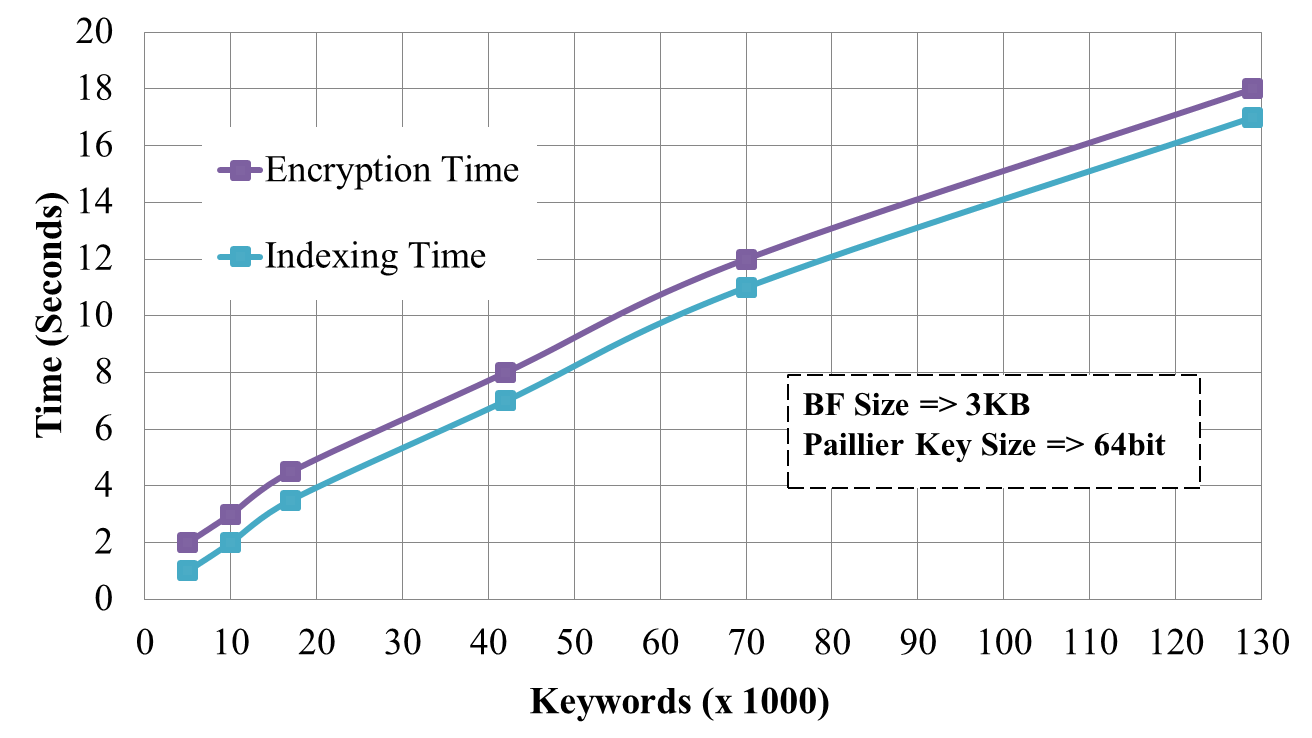
\includegraphics[width=3.5in]{figures/indexing_encryption_time.png}
  \caption{Index Generation Time}
  \label{fig:Index-Generation-Time}
\end{figure}

Paillier key size and bloom filter size both have a substantial impact on index file size. 
With the increase of bloom filter size, the false positive rate decreases but the size of each
index entry increases. The indexing time also increases, mainly because it takes longer
to upload a larger bloom filter to the cloud. 
A larger Paillier key size can help strengthen system security. However, with
increasing Paillier key size, index file size also increases proportionally and
out experiments shows that index size increases linearly with Paillier key size.

\subsection{Search Performance}

Search performance is evaluated in terms of data returned by a query, response
time, CPU cycles used to process a search request and the cost(\$) CSP will
charge for search queries. 
For private term matching and data returned, our implementation demonstrates
that by using our compression algorithm, data returned to the client
is 95\% less than traditional approaches and remains constant even when the size
of the bloom filter increases. This is shown in Figure \ref{fig:compress}.

\begin{figure}[h!]
  \centering
  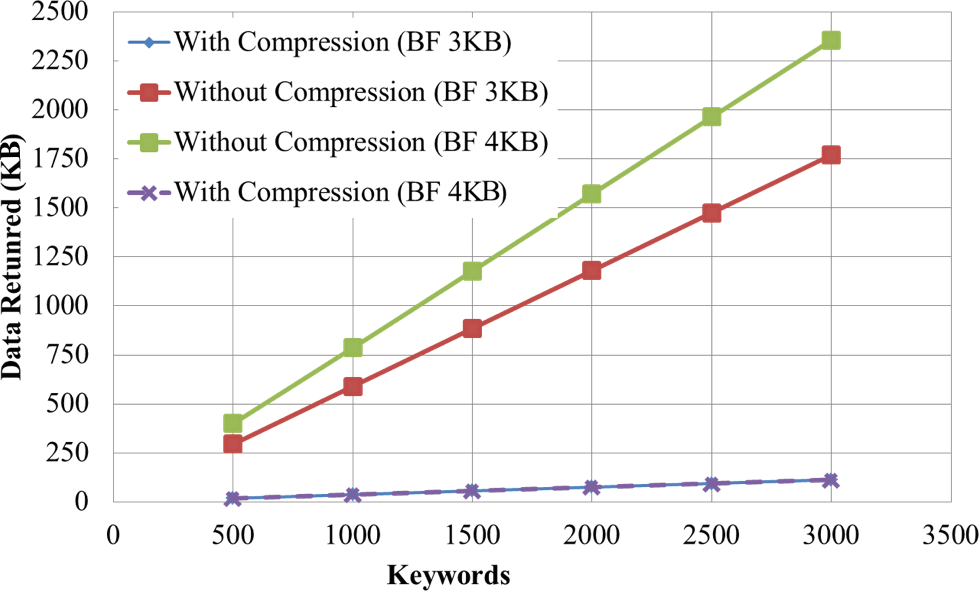
\includegraphics[width= 3.5in]{figures/comp_compare.png}
  \caption{Data returned by a search query: compressed vs uncompressed results}
  \label{fig:compress}
\end{figure}

We also measure the time it takes to extract the matching bloom filter values
from the compressed responses.
Table \ref{tab:search_response_time} show the results. As expected,
the extraction time increases linearly with the keyword count
on the server. The reason is that we add more keywords
keywords by adding more documents to the dataset and each document
has its own bloom filter index associated with it.

\begin{table}[th!]
\centering
\caption{Response time increases almost linearly with keyword count.}
\label{tab:search_response_time}
\begin{tabular}{| c | c | }
\hline
Keyword Count & Response Extraction Time (ms) \\
\hline
500  &  60 \\
1000 &  125 \\
1500 &  185 \\
2000 &  250 \\
2500 &  310 \\
3000 &  370 \\
\hline
\end{tabular}


\end{table}


\subsection{Cost Estimation and Response Times}

Finally, we evaluate the cost(\$) that CSP will charge to data owners for search
queries with partial matching. 
Our results, shown in Figure \ref{fig:cost_single_query}, demonstrate that a query
searching for a single keyword in a dataset having 500-3500 index entries will cost only \$0.000002 to \$0.00002 per 1000 similar
queries. Due to the sliding window bloom filter approach, 
all of the metrics increase only linearly ($O(n)$) with the number
of keywords on the server. This is substantially better than using a naive algorithm 
for partial matching, which would result in $O(nm)$ time complexity 
for $n$ keywords that are on average $m$ characters long. Crucially,
privacy is preserved throughout the search process because data is never
decrypted at the cloud or by any other untrusted system.

We obtained these cost metrics from Google App Engine logs for each data point. In
each log entry \emph{ms}, \emph{cpu\_ms} and \emph{cpm\_usd} depicts the wallclock response
time for a request, the \emph{normalized} CPU time needed to process the
request, and cost(\$) incurred for 1000 similar requests~\cite{google_cloud_logs}.


\begin{figure}
  \centering
  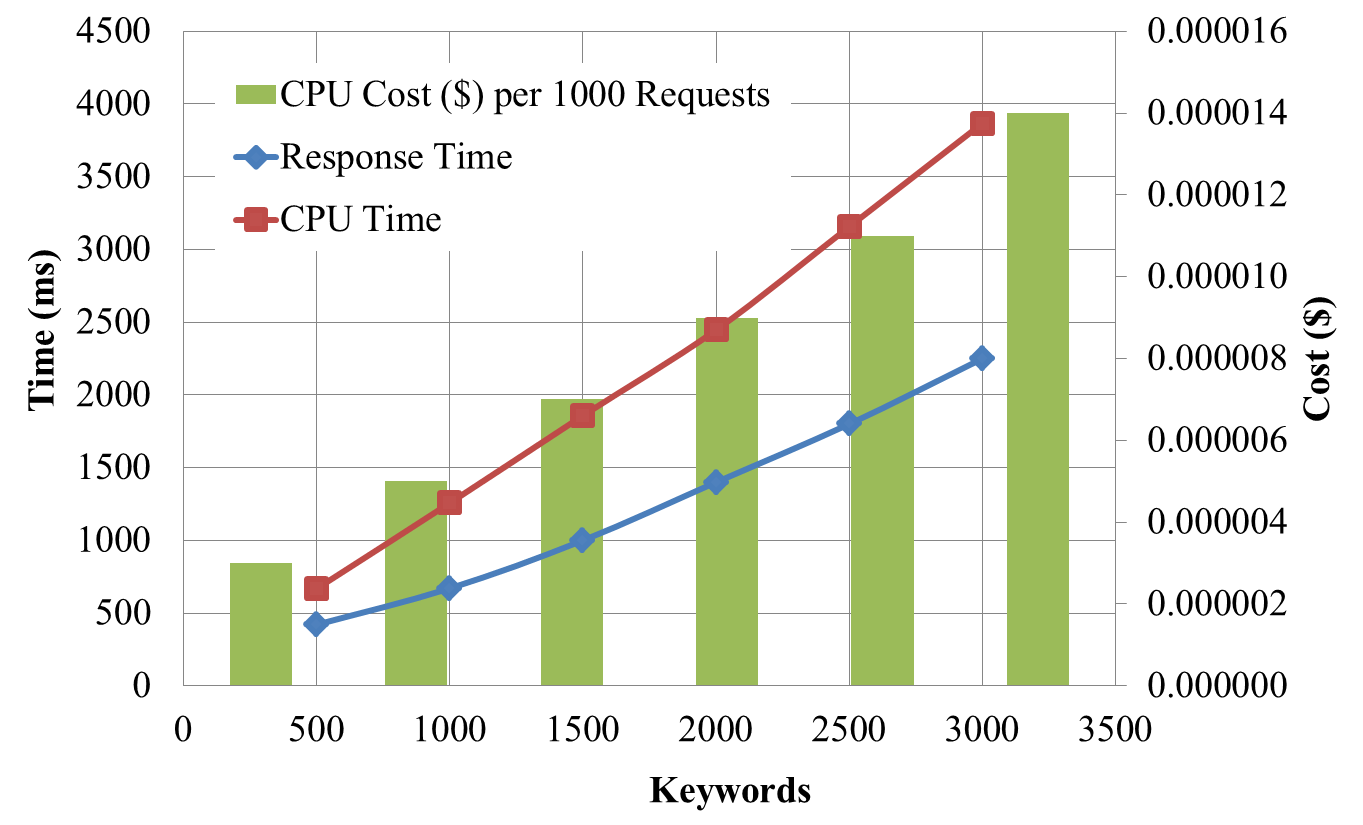
\includegraphics[width= 3.6in]{figures/cost_keywords_graph.png}
  \caption{Searching Cost(\$) with Single Keyword Query}
  \label{fig:cost_single_query}
\end{figure}

\section{Future Work}
\label{sec:futurework}

While homomorphic encryption allows us to implement this system effectively, 
it is still much slower than symmetric and public-key encryption.
In this paper, we have demonstrated and tested our system with a comparatively 
small dataset. With larger amounts of data, the indexer will likely take 
much more time to generate the
encrypted index. To optimize indexing time we can
utilize scalable systems like Hadoop~\cite{hadoop} for indexing
purposes. In addition, it would be useful to explore CryptDB and MONOMI as
ways to improve the performance of both the indexer and the searcher.


\section{Conclusion}
\label{sec:conclusion}

In this paper, we presented a privacy-aware similarity-based searching scheme
with reduced communication cost over encrypted data residing in an untrusted
cloud domain. Using a novel compression 
algorithm, our system avoids the need to send the bloom filter based index back to the 
user, reducing communication costs by over 95\%.
By using homomorphic encryption for index files, a cloud service provider can not learn the contents of 
the data files, the index files or the search queries. Furthermore, it cannot 
discern patterns from incoming queries. Moreover, unlike most existing techniques, our
proposed system supports similarity-based searching in addition to exact matching.
Since our system does not rely on trapdoors, it allows end users to formulate
arbitrary queries and perform search. 

 
\bibliographystyle{IEEEtran}
\bibliography{ias}



\end{document}
